% Titre : fonctions
% Filiere : BCPST
% Difficulte : 
% Type : TD 
% Categories :fonctions
% Subcategories : 
% Keywords : fonctions




\begin{exercice} 
\`{A} l'aide d'une \'etude de fonction, d\'emontrer les in\'egalit\'es suivantes:
\begin{enumerate}
\item $\forall \ddp x>0,\ x-\frac{x^2}{2}\leq \ln{(1+x)}\leq x$
\item $\forall \ddp x\in\R^+$: $e^x-\ddp\frac{x^2}{2}\geq 1$.
\end{enumerate}
\end{exercice}


\%\%\%\%\%\%\%\%\%\%\%\%\%\%\%\%\%\%\%\%
\%\%\%\%\%\%\%\%\%\%\%\%\%\%\%\%\%\%\%\%
\%\%\%\%\%\%\%\%\%\%\%\%\%\%\%\%\%\%\%\%



\begin{correction}  \; \textbf{Utilisation d'une \'etude de fonction.}\\
\begin{enumerate}
\item \textbf{Montrons que $\mathbf{\forall x>0,\ddp\ x-\frac{x^2}{2}\leq \ln{(1+x)}\leq x}$:}\\
\noindent On d\'emontre l'in\'egalit\'e en deux temps.
\begin{itemize}
\item[$\bullet$] Montrons d'abord que pour tout $x>0$: $x-\ddp\frac{x^2}{2}\leq \ln{(1+x)}$:\\
\noindent On pose pour cela la fonction $f(x)=\ln{(1+x)}-x+\ddp\frac{x^2}{2}$. Cette fonction est bien d\'efinie sur $\R^{+}$ et elle est d\'erivable sur $\R^{+}$ comme compos\'ee et somme de fonctions d\'erivables. On obtient pour tout $x\geq  0$: $f^{\prime}(x)=\ddp\frac{1}{1+x}-1+x=\ddp\frac{x^2}{1+x}$. Comme on est sur $\R^{+}$, on a: $f^{\prime}(x)\geq 0$. On obtient donc les variations suivantes en utilisant le fait que $f(0)=0$: 
\begin{center}
\begin{tikzpicture}
 \tkzTabInit[espcl=5]{ $x$          /1,
       $f^{\prime}(x)$    /1,
       $f(x)$            /2}
     { $0$ ,$+\infty$}
  \tkzTabLine {,$+$,}
  \tkzTabVar{
       -/ $0$        /,
       +/           /
                      }
\end{tikzpicture}
\end{center}
Ainsi $0$ est le minimum de $f$ sur $\R^{+}$ et on obtient bien que pour tout $x>0$: $\ln{(1+x)}-x+\ddp\frac{x^2}{2}\geq 0$, \`{a} savoir $x-\ddp\frac{x^2}{2} \leq \ln{(1+x)}$.
\item[$\bullet$] On montre de m\^eme la deuxi\`eme in\'egalit\'e en \'etudiant la fonction $g(x)=\ln{(1+x)}-x$.
\end{itemize}
%---
\item \textbf{Montrons que $\mathbf{\forall x\in\R^+,\ e^x - \ddp \frac{x^2}{2}\geq 1}$:}\\
\noindent Pour tout $x\in\R^+$, on pose $f(x)=e^x-\ddp \frac{x^2}{2}-1$. La fonction $f$ est d\'efinie et d\'erivable sur $\R$ comme somme de fonctions d\'efinies et d\'erivables. On a, pour tout $x\in\R$,
$$f^{\prime}(x)=e^x-x.$$
Or on a montr\'e dans le cours (il faudrait refaire le raisonnement) que l'on a $e^x \geq x+1$ pour tout $x \in \R$, donc on a $f'(x) \geq 0$ sur $\R^+$. On obtient alors le tableau de variation suivant
\begin{center}
\begin{tikzpicture}
 \tkzTabInit{ $x$          /1,
       $f^{\prime}(x)$    /1,
       $f(x)$            /2}
     { $0$ ,$+\infty$}
  \tkzTabLine {,$+$,}
  \tkzTabVar{
        -/$0$           /,
       +/ $+\infty$          /
                      }
\end{tikzpicture}
\end{center}
Justifions les limites aux bornes: on a: $f(0)=e^0-0-1=0$. L'\'etude en $+\infty$ fait appara\^{i}tre une forme ind\'etermin\'ee. Pour lever l'ind\'etermination, on met en facteur le terme dominant \`{a} savoir $e^x$ et on obtient ainsi: $f(x)=e^x\left( 1-\ddp\frac{x^2}{2e^x}-\ddp\frac{1}{e^x}  \right)$. Par croissance compar\'ee, on sait que $\lim\limits_{x\to +\infty} \ddp\frac{x^2}{2e^x}=0$. Ainsi par quotient, somme et produit de limite, on obtient que $\lim\limits_{x\to +\infty}  f(x)=+\infty$.\\
\noindent Ainsi, $0$ est le minimum de $f$ atteint en $x=0$ et donc la fonction $f$ est toujours positive ou nulle. Ainsi, on a bien 
$$\fbox{$ \forall x\in \R,\ e^x\geq \ddp \frac{x^2}{2}+1. $}$$
%\item \textbf{Montrons que $\mathbf{\forall x\in\R,\ e^x\geq x+1}$:}\\
%\noindent \'Etude de l'in\'equation avec l'exponentielle.
%Pour tout $x\in\R$, on pose $f(x)=e^x-x-1$. La fonction $f$ est d\'efinie et d\'erivable sur $\R$ comme somme alg\'ebrique de fonctions d\'efinies et d\'erivables. On a, pour tout $x\in\R$,
%$$f^{\prime}(x)=e^x-1.$$
%\'Etudions donc le signe de $e^x-1$:
%$$e^x-1>0\Leftrightarrow e^x>e^0\Leftrightarrow x>0$$
%car la fonction $\ln{}$ est strictement croissante sur $\R^{+\star}$.
%On obtient alors le tableau de variation suivant
%\begin{center}
%\begin{tikzpicture}
% \tkzTabInit{ $x$          /,%
%      % $\sin{x}$     /,%
%      % $\sin{(2x)}$       /,
%       $f^{\prime}(x)$    /,
%       $f(x)$            /2}%
%     { $-\infty$ , $0$ ,$+\infty$}%
%  \tkzTabLine {,$-$,0,$+$,}%
%  %\tkzTabLine{ 0,$+$,0,$-$,0}
%  % \tkzTabLine{ 0,$+$,0,$-$,0}
%  \variation{
%     % {-/ $1$       /,%
%       +/ $+\infty$        /,
%        -/$0$           /,%
%       +/ $+\infty$          /
%                      }
%\end{tikzpicture}
%\end{center}
%Justifions les limites aux bornes: on a: $f(0)=e^0-1=0$. De plus $\lim\limits_{x\to -\infty} f(x)=+\infty$ comme sommes de limites. L'\'etude en $+\infty$ fait appara\^{i}tre une forme ind\'etermin\'ee. Pour lever l'ind\'etermination, on met en facteur le terme dominant \`{a} savoir $e^x$ et on obtient ainsi: $f(x)=e^x\left( 1-\ddp\frac{x}{e^x}-\ddp\frac{1}{e^x}  \right)$. Par croissance compar\'ee, on sait que $\lim\limits_{x\to +\infty} \ddp\frac{x}{e^x}=0$. Ainsi par quotient, somme et produit de limite, on obtient que $\lim\limits_{x\to +\infty}  f(x)=+\infty$.\\
%\noindent Ainsi, $0$ est le minimum de $f$ atteint en $x=0$ et donc la fonction $f$ est toujours positive ou nulle. Ainsi, on a bien 
%$$\fbox{$ \forall x\in \R,\ e^x\geq x+1. $}$$
%\item \textbf{Montrons que $\mathbf{\forall x\in\R^+,\ \sin{x}\leq x}$:}\\
%\noindent Pour cela on pose pour tout $x\in\R^+$: $f(x)=\sin{(x)}-x$. On va alors \'etudier les variations de cette fonction afin de montrer qu'elle est toujours n\'egative sur $\R^+$.
%\begin{itemize}
%\item[$\bullet$] La fonction $f$ est bien d\'efinie sur $\R$ donc en particulier sur $\R^+$.
%\item[$\bullet$] La fonction $f$ est d\'erivable sur $\R^+$ comme somme de fonctions d\'erivables. Et pour tout $x\in\R^+$, on a: $f^{\prime}(x)=\cos{(x)}-1$. Comme pour tout $x\in\R$, on a: $-1\leq \cos{(x)}\leq 1$, on obtient en particulier que pour tout $x\in\R^+$: $\cos{(x)}-1\leq 0$. Ainsi pour tout $x\in\R^+$: $f^{\prime}(x)\leq 0$.
%\item[$\bullet$] Tableau de variation:
%\begin{center}
%\begin{tikzpicture}
% \tkzTabInit[espcl=5]{ $x$          /,%
%      % $\sin{x}$     /,%
%      % $\sin{(2x)}$       /,
%       $f^{\prime}(x)$    /,
%       $f(x)$            /2}%
%     {$0$ ,$+\infty$}%
%  \tkzTabLine {,$-$,}%
%  %\tkzTabLine{ 0,$+$,0,$-$,0}
%  % \tkzTabLine{ 0,$+$,0,$-$,0}
%  \variation{
%     % {-/ $1$       /,%
%       +/ $0$        /,
%        -/           /%
%      % +/ $+\infty$          /
%                      }
%\end{tikzpicture}
%\end{center}
%\item[$\bullet$] Ainsi 0 est le maximum de $f$ sur $\R^+$ atteint en $x=0$. Donc pour tout $x\in\R^+$: $f(x)\leq 0$ ce qui est bien \'equivalent \`{a}: \fbox{$ \forall x\in\R^+,\ \sin{(x)}\leq x .$}
%\end{itemize}
\end{enumerate}
\end{correction}